
\bta{2017}


\section{Use of English}

\noindent
\textbf{Directions:}
Read the following text. Choose the best word (s) for each numbered blank
and mark A, B, C or D on the ANSWER SHEET. (10 points)


\TiGanSpace


Could a hug a day keep the doctor away? The answer may be a resounding
``yes!'' \cloze helping you feel close and \cloze to
people you care about, it turns out that hugs can bring a \cloze
of health benefits to your body and mind. Believe it or not, a warm
embrace might even help you \cloze getting sick this winter.

In a recent study \cloze over 400 healthy adults, researchers
from Carnegie Mellon University in Pennsylvania examined the effects of
perceived social support and the receipt of hugs \cloze the
participants' susceptibility to developing the common cold after being
\cloze to the virus. People who perceived greater social support
were less likely to come \cloze with a cold, and the researchers
\cloze that the stress-reducing effects of hugging \cloze
about 32 percent of that beneficial effect. \cloze among those
who got a cold, the ones who felt greater social support and received
more frequent hugs had less severe \cloze.

``Hugging protects people who are under stress from the \cloze
risk for colds that's usually \cloze with stress,'' notes
Sheldon Cohen, a professor of psychology at Carnegie. Hugging ``is a
marker of intimacy and helps \cloze the feeling that others are
there to help \cloze difficulty.''

Some experts \cloze the stress-reducing, health-related
benefits of hugging to the release of oxytocin, often called ``the
bonding hormone'' \cloze it promotes attachment in
relationships, including that between mothers and their newborn babies.
Oxytocin is made primarily in the central lower part of the brain, and
some of it is released into the bloodstream. But some of it
\cloze in the brain, where it \cloze mood, behavior and
physiology.


\newpage

\begin{enumerate}
	%\renewcommand{\labelenumi}{\arabic{enumi}.}
	% A(\Alph) a(\alph) I(\Roman) i(\roman) 1(\arabic)
	%设定全局标号series=example	%引用全局变量resume=example
	%[topsep=-0.3em,parsep=-0.3em,itemsep=-0.3em,partopsep=-0.3em]
	%可使用leftmargin调整列表环境左边的空白长度 [leftmargin=0em]
	\item


\fourchoices
{Unlike}
{Besides}
{Throughout}
{Despite}




\item


\fourchoices
{equal}
{restricted}
{connected}
{inferior}




\item


\fourchoices
{host}
{view}
{lesson}
{choice}




\item


\fourchoices
{recall}
{forget}
{avoid}
{keep}




\item

\fourchoices
{collecting}
{affecting}
{guiding}
{involving}


\item


\fourchoices
{on}
{in}
{at}
{of}




\item


\fourchoices
{devoted}
{exposed}
{lost}
{attracted}




\item


\fourchoices
{along}
{across}
{down}
{out}




\item


\fourchoices
{imagined}
{denied}
{doubted}
{calculated}




\item


\fourchoices
{served}
{explained}
{restored}
{required}




\item


\fourchoices
{Thus}
{Still}
{Rather}
{Even}




\item


\fourchoices
{defeats}
{symptoms}
{errors}
{tests}




\item

\fourchoices
{highlighted}
{minimized}
{controlled}
{increased}



\item

\fourchoices
{associated}
{equipped}
{presented}
{compared}


\item


\fourchoices
{assess}
{moderate}
{generate}
{record}




\item

\fourchoices
{in the face of}
{in the form of}
{in the name of}
{in the way of}


\item


\fourchoices
{attribute}
{commit}
{transfer}
{return}




\item


\fourchoices
{unless}
{because}
{though}
{until}




\item


\fourchoices
{vanishes}
{emerges}
{remains}
{decreases}




\item

\fourchoices
{experiences}
{combines}
{justifies}
{influences}



\end{enumerate}


\hfill

\section{Reading Comprehension}


\noindent
\textbf{Part A}\\
\textbf{Directions:}\\
Read the following four texts. Answer the questions below each text by
choosing A, B, C or
D. Mark your answers on the ANSWER SHEET. (40 points)

\newpage
\subsection{Text 1}


First two hours, now three hours---this is how far in advance
authorities are recommending people show up to catch a domestic flight,
at least at some major U.S. airports with increasingly massive security
lines.

Americans are willing to tolerate time-consuming security procedures in
return for increased safety. The crash of EgyptAir Flight 804, which
terrorists may have downed over the Mediterranean Sea, provides another
tragic reminder of why. But demanding too much of air travelers or
providing too little security in return undermines public support for
the process. And it should: Wasted time is a drag on Americans'
economic and private lives, not to mention infuriating.

Last year, the Transportation Security Administration (TSA) found in a
secret check that undercover investigators were able to sneak
weapons---both fake and real---past airport security nearly every time
they tried. Enhanced security measures since then, combined with a rise
in airline travel due to the improving economy and low oil prices, have
resulted in long waits at major airports such as Chicago's O'Hare
International. It is not yet clear how much more effective airline
security has become---but the lines are obvious.

Part of the issue is that the government did not anticipate the steep
increase in airline travel, so the TSA is now rushing to get new
screeners on the line. Part of the issue is that airports have only so
much room for screening lanes. Another factor may be that more people
are trying to overpack their carry-on bags to avoid checked-baggage
fees, though the airlines strongly dispute this.

There is one step the TSA could take that would not require remodeling
airports or rushing to hire: Enroll more people in the PreCheck program.
PreCheck is supposed to be a win-win for travelers and the TS
A.
Passengers who pass a background check are eligible to use
\uline{expedited} screening lanes. This allows the TSA to focus on
travelers who are higher risk, saving time for everyone involved. The
TSA wants to enroll 25 million people in PreCheck.

It has not gotten anywhere close to that, and one big reason is sticker
shock: Passengers must pay \$85 every five years to process their
background checks. Since the beginning, this price tag has been
PreCheck's fatal flaw. Upcoming reforms might bring the price to a more
reasonable level. But Congress should look into doing so directly, by
helping to finance PreCheck enrollment or to cut costs in other ways.

The TSA cannot continue diverting resources into underused PreCheck
lanes while most of the traveling public suffers in unnecessary lines.
It is long past time to make the program work.

\begin{enumerate}[resume]
	%\renewcommand{\labelenumi}{\arabic{enumi}.}
	% A(\Alph) a(\alph) I(\Roman) i(\roman) 1(\arabic)
	%设定全局标号series=example	%引用全局变量resume=example
	%[topsep=-0.3em,parsep=-0.3em,itemsep=-0.3em,partopsep=-0.3em]
	%可使用leftmargin调整列表环境左边的空白长度 [leftmargin=0em]
	\item
The crash of EgyptAir Flight 804 is mentioned to \lineread.


\fourchoices
{explain Americans' tolerance of current security checks}
{stress the urgency to strengthen security worldwide}
{highlight the necessity of upgrading major U.S. airports}
{emphasize the importance of privacy protection}



\item
Which of the following contributes to long waits at major airports?


\fourchoices
{New restrictions on carry-on bags.}
{The declining efficiency of the TSA.}
{An increase in the number of travelers.}
{Frequent unexpected secret checks.}



\item
The word ``expedited'' (Line 4, Para. 5) is closest in meaning to \lineread.


\fourchoices
{quieter}
{cheaper}
{wider}
{faster}





\item
One problem with the PreCheck program is  \lineread.


\fourchoices
{a dramatic reduction of its scale}
{its wrongly-directed implementation}
{the government's reluctance to back it}
{an unreasonable price for enrollment}


\item
Which of the following would be the best title for the text?


\fourchoices
{Less Screening for More Safety}
{PreCheck---a Belated Solution}
{Getting Stuck in Security Lines}
{Underused PreCheck Lanes}


\end{enumerate}


\newpage
\subsection{Text 2}


``The ancient Hawaiians were astronomers,'' wrote Queen Liliuokalani,
Hawaii's last reigning monarch, in 1897. Star watchers were among the
most esteemed members of Hawaiian society. Sadly, all is not well with
astronomy in Hawaii today. Protests have erupted over construction of
the Thirty Meter Telescope (TMT), a giant observatory that promises to
revolutionize humanity's view of the cosmos.

At issue is the TMT's planned location on Mauna Kea, a dormant volcano
worshiped by some Hawaiians as the \emph{piko}, that connects the
Hawaiian Islands to the heavens. But Mauna Kea is also home to some of
the world's most powerful telescopes. Rested in the Pacific Ocean,
Mauna Kea's peak rises above the bulk of our planet's dense atmosphere,
where conditions allow telescopes to obtain images of unsurpassed
clarity.

Opposition to telescopes on Mauna Kea is nothing new. A small but
vocal group of Hawaiians and environmentalists have long viewed their
presence as disrespect for sacred land and a painful reminder of the
occupation of what was once a sovereign nation.

Some blame for the current controversy belongs to astronomers. In
their eagerness to build bigger telescopes, they forgot that science is
not the only way of understanding the world. They did not always
prioritize the protection of Mauna Kea's fragile ecosystems or its
holiness to the islands' inhabitants. Hawaiian culture is not a relic
of the past; it is a living culture undergoing a renaissance today.

Yet science has a cultural history, too, with roots going back to the
dawn of civilization. The same curiosity to find what lies beyond the
horizon that first brought early Polynesians to Hawaii's shores inspires
astronomers today to explore the heavens. Calls to disassemble all
telescopes on Mauna Kea or to ban future development there ignore the
reality that astronomy and Hawaiian culture both seek to answer big
questions about who we are, where we come from and where we are going.
Perhaps that is why we explore the starry skies, as if answering a
primal calling to know ourselves and our true ancestral homes.

The astronomy community is making compromises to change its use of
Mauna Kea. The TMT site was chosen to minimize the telescope's
visibility around the island and to avoid archaeological and
environmental impact. To limit the number of telescopes on Mauna Kea,
old ones will be removed at the end of their lifetimes and their sites
returned to a natural state. There is no reason why everyone cannot be
welcomed on Mauna Kea to embrace their cultural heritage and to study
the stars.

\begin{enumerate}[resume]
	%\renewcommand{\labelenumi}{\arabic{enumi}.}
	% A(\Alph) a(\alph) I(\Roman) i(\roman) 1(\arabic)
	%设定全局标号series=example	%引用全局变量resume=example
	%[topsep=-0.3em,parsep=-0.3em,itemsep=-0.3em,partopsep=-0.3em]
	%可使用leftmargin调整列表环境左边的空白长度 [leftmargin=0em]
	\item
Queen Liliuokalani's remark in Paragraph 1 indicates \lineread.


\fourchoices
{her conservative view on the historical role of astronomy}
{the importance of astronomy in ancient Hawaiian society}
{the regrettable decline of astronomy in ancient times}
{her appreciation of star watchers' feats in her time}




\item
Mauna Kea is deemed as an ideal astronomical site due to \lineread.


\fourchoices
{its geographical features}
{its protective surroundings}
{its religious implications}
{its existing infrastructure}


\item
The construction of the TMT is opposed by some locals partly because \lineread.


\fourchoices
{it may risk ruining their intellectual life}
{it reminds them of a humiliating history}
{their culture will lose a chance of revival}
{they fear losing control of Mauna Kea}




\item
It can be inferred from Paragraph 5 that progress in today's
astronomy \lineread.

\fourchoices
{is fulfilling the dreams of ancient Hawaiians}
{helps spread Hawaiian culture across the world}
{may uncover the origin of Hawaiian culture}
{will eventually soften Hawaiians' hostility}


\item
The author's attitude toward choosing Mauna Kea as the TMT site is
one of \lineread.


\fourchoices
{severe criticism}
{passive acceptance}
{slight hesitancy}
{full approval}



\end{enumerate}


\newpage
\subsection{Text 3}


Robert F. Kennedy once said that a country's GDP measures ``everything
except that which makes life worthwhile.'' With Britain voting to leave
the European Union, and GDP already predicted to slow as a result, it is
now a timely moment to assess what he was referring to.

The question of GDP and its usefulness has annoyed policymakers for
over half a century. Many argue that it is a flawed concept. It
measures things that do not matter and misses things that do. By most
recent measures, the UK's GDP has been the envy of the Western world,
with record low unemployment and high growth figures. If everything was
going so well, then why did over 17 million people vote for Brexit,
despite the warnings about what it could do to their country's economic
prospects?

A recent annual study of countries and their ability to convert growth
into well-being sheds some light on that question. Across the 163
countries measured, the UK is one of the poorest performers in ensuring
that economic growth is translated into meaningful improvements for its
citizens. Rather than just focusing on GDP, over 40 different sets of
criteria from health, education and civil society engagement have been
measured to get a more rounded assessment of how countries are
performing.

While all of these countries face their own challenges, there are a
number of consistent themes. Yes, there has been a budding economic
recovery since the 2008 global crash, but in key indicators in areas
such as health and education, major economies have continued to decline.
Yet this isn't the case with all countries. Some relatively poor
European countries have seen huge improvements across measures including
civil society, income equality and the environment.

This is a lesson that rich countries can learn: When GDP is no longer
regarded as the sole measure of a country's success, the world looks
very different.

So, what Kennedy was referring to was that while GDP has been the most
common method for measuring the economic activity of nations, as a
measure, it is no longer enough. It does not include important factors
such as environmental quality or education outcomes---all things that
contribute to a person's sense of well-being.

The sharp hit to growth predicted around the world and in the UK could
lead to a decline in the everyday services we depend on for our
well-being and for growth. But policymakers who refocus efforts on
improving well-being rather than simply worrying about GDP figures could
avoid the forecasted doom and may even see progress.


\begin{enumerate}[resume]
	%\renewcommand{\labelenumi}{\arabic{enumi}.}
	% A(\Alph) a(\alph) I(\Roman) i(\roman) 1(\arabic)
	%设定全局标号series=example	%引用全局变量resume=example
	%[topsep=-0.3em,parsep=-0.3em,itemsep=-0.3em,partopsep=-0.3em]
	%可使用leftmargin调整列表环境左边的空白长度 [leftmargin=0em]
	\item
Robert F. Kennedy is cited because he  \lineread.


\fourchoices
{praised the UK for its GDP}
{identified GDP with happiness}
{misinterpreted the role of GDP}
{had a low opinion of GDP}



\item
It can be inferred from Paragraph 2 that  \lineread.


\fourchoices
{the UK is reluctant to remold its economic pattern}
{the UK will contribute less to the world economy}
{GDP as the measure of success is widely defied in the UK}
{policymakers in the UK are paying less attention to GDP}


\item
Which of the following is true about the recent annual study?


\fourchoices
{It excludes GDP as an indicator.}
{It is sponsored by 163 countries.}
{Its criteria are questionable.}
{Its results are enlightening.}


\item
 In the last two paragraphs, the author suggests that \lineread.


\fourchoices
{the UK is preparing for an economic boom}
{high GDP foreshadows an economic decline}
{it is essential to consider factors beyond GDP}
{it requires caution to handle economic issues}



\item
Which of the following is the best title for the text?


\fourchoices
{High GDP But Inadequate Well-being, a UK Lesson}
{GDP Figures, a Window on Global Economic Health}
{Robert F. Kennedy, a Terminator of GDP}
{Brexit, the UK's Gateway to Well-being}
	
\end{enumerate}


\newpage
\subsection{Text 4}


In a rare unanimous ruling, the US Supreme Court has overturned the
corruption conviction of a former Virginia governor, Robert McDonnell.
\uline{But it did so while holding its nose at the ethics of his
	conduct}, which included accepting gifts such as a Rolex watch and a
Ferrari automobile from a company seeking access to government.

The high court's decision said the judge in Mr. McDonnell's trial
failed to tell a jury that it must look only at his ``official acts,''
or the former governor's decisions on ``specific'' and ``unsettled''
issues related to his duties.

Merely helping a gift-giver gain access to other officials, unless done
with clear intent to pressure those officials, is not corruption, the
justices found.

The court did suggest that accepting favors in return for opening doors
is ``distasteful'' and ``nasty.'' But under anti-bribery laws, proof
must be made of concrete benefits, such as approval of a contract or
regulation. Simply arranging a meeting, making a phone call, or hosting
an event is not an ``official act.''

The court's ruling is legally sound in defining a kind of favoritism
that is not criminal. Elected leaders must be allowed to help
supporters deal with bureaucratic problems without fear of prosecution
of bribery. ``The basic compact underlying representative government,''
wrote Chief Justice John Roberts for the court, ``assumes that public
officials will hear from their constituents and act on their concerns.''

But the ruling reinforces the need for citizens and their elected
representatives, not the courts, to ensure equality of access to
government. Officials must not be allowed to play favorites in
providing information or in arranging meetings simply because an
individual or group provides a campaign donation or a personal gift.
This type of integrity requires well-enforced laws in government
transparency, such as records of official meetings, rules on lobbying,
and information about each elected leader's source of wealth.

Favoritism in official access can fan public perceptions of corruption.
But it is not always corruption. Rather officials must avoid double
standards, or different types of access for average people and the
wealthy. If connections can be bought, a basic premise of democratic
society---that all are equal in treatment by government---is
undermined. Good governance rests on an understanding of the inherent
worth of each individual.

The court's ruling is a step forward in the struggle against both
corruption and official favoritism.

\begin{enumerate}[resume]
	%\renewcommand{\labelenumi}{\arabic{enumi}.}
	% A(\Alph) a(\alph) I(\Roman) i(\roman) 1(\arabic)
	%设定全局标号series=example	%引用全局变量resume=example
	%[topsep=-0.3em,parsep=-0.3em,itemsep=-0.3em,partopsep=-0.3em]
	%可使用leftmargin调整列表环境左边的空白长度 [leftmargin=0em]
	\item
The underlined sentence (Para. 1) most probably shows that the court \lineread.

\fourchoices
{avoided defining the extent of McDonnell's duties}
{made no compromise in convicting McDonnell}
{was contemptuous of McDonnell's conduct}
{refused to comment on McDonnell's ethics}



\item
 According to Paragraph 4, an official act is deemed corruptive only
if it involves \lineread.


\fourchoices
{concrete returns for gift-givers}
{sizable gains in the form of gifts}
{leaking secrets intentionally}
{breaking contracts officially}



\item
The court's ruling is based on the assumption that public officials
are \lineread.


\fourchoices
{allowed to focus on the concerns of their supporters}
{qualified to deal independently with bureaucratic issues}
{justified in addressing the needs of their constituents}
{exempt from conviction on the charge of favoritism}


\item
Well-enforced laws in government transparency are needed to \lineread.


\fourchoices
{awaken the conscience of officials}
{guarantee fair play in official access}
{allow for certain kinds of lobbying}
{inspire hopes in average people}



\item
The author's attitude toward the court's ruling is \lineread.


\fourchoices
{sarcastic}
{tolerant}
{skeptical}
{supportive}





\end{enumerate}

\newpage

\noindent
\textbf{Part B}\\
\textbf{Directions:}\\
The following paragraphs are given in a wrong order. For questions
41-45, you are required to reorganize these paragraphs into a coherent
text by choosing from the list A-G and filling them into the numbered
boxes. Paragraphs B and D have been correctly placed. Mark your
answers on the ANSWER SHEET. (10 points)


\begin{listmatch}


\item 
The first published sketch, ``A Dinner at Poplar Walk'' brought tears
to Dickens's eyes when he discovered it in the pages of \emph{The Monthly Magazine}. From then on his sketches, which appeared under the
pen name ``Boz'' in \emph{The Evening Chronicle}, earned him a modest
reputation.


\item 
The runaway success of \emph{The Pickwick Papers}, as it is generally
known today, secured Dickens's fame. There were Pickwick coats and
Pickwick cigars, and the plump, spectacled hero, Samuel Pickwick, became
a national figure.


\item 
Soon after \emph{Sketches by Boz} appeared, a publishing firm
approached Dickens to write a story in monthly installments, as a
backdrop for a series of woodcuts by the then-famous artist Robert
Seymour, who had originated the idea for the story. With characteristic
confidence, Dickens successfully insisted that Seymour's pictures
illustrate his own story instead. After the first installment, Dickens
wrote to the artist and asked him to correct a drawing Dickens felt was
not faithful enough to his prose. Seymour made the change, went into his
backyard, and expressed his displeasure by committing suicide. Dickens
and his publishers simply pressed on with a new artist. The comic novel,
\emph{The Posthumous Papers of the Pickwick Club}, appeared serially in
1836 and 1837 and was first published in book form in 1837.


\item 
Charles Dickens is probably the best-known and, to many people, the
greatest English novelist of the 19th century. A moralist, satirist, and
social reformer, Dickens crafted complex plots and striking characters
that capture the panorama of English society.


\item 
Soon after his father's release from prison, Dickens got a better job
as errand boy in law offices. He taught himself shorthand to get an even
better job later as a court stenographer and as a reporter in
Parliament. At the same time, Dickens, who had a reporter's eye for
transcribing the life around him, especially anything comic or odd,
submitted short sketches to obscure magazines.


\item 
Dickens was born in Portsmouth, on England's southern coast. His
father was a clerk in the British Navy pay office---a respectable
position, but with little social status. His paternal grandparents, a
steward and a housekeeper, possessed even less status, having been
servants, and Dickens later concealed their background. Dicken's mother
supposedly came from a more respectable family. Yet two years before
Dicken's birth, his mother's father was caught stealing and fled to
Europe, never to return. The family's increasing poverty forced Dickens
out of school at age 12 to work in Warren's Blacking Warehouse, a
shoe-polish factory, where the other working boys mocked him as ``the
young gentleman.'' His father was then imprisoned for debt. The
humiliations of his father's imprisonment and his labor in the blacking
factory formed Dickens's greatest wound and became his deepest secret.
He could not confide them even to his wife, although they provide the
unacknowledged foundation of his fiction.


\item 
After \emph{Pickwick}, Dickens plunged into a bleaker world. In
\emph{Oliver Twist}, he traces an orphan's progress from the workhouse
to the criminal slums of London. \emph{Nicholas Nickleby}, his next
novel, combines the darkness of \emph{Oliver Twist} with the sunlight of
\emph{Pickwick}. The popularity of these novels consolidated Dickens' as
a nationally and internationally celebrated man of letters.



\end{listmatch}


\[ 
\begin{tabular}{|c|}
	\hline
	D \\
	\hline
\end{tabular}
\rightarrow
\begin{tabular}{|c|c|}
	\hline
	41. &  \hspace{1.5em} \\
	\hline
\end{tabular}
\rightarrow
\begin{tabular}{|c|c|}
	\hline
	42. &  \hspace{1.5em} \\
	\hline
\end{tabular}
\rightarrow
\begin{tabular}{|c|c|}
	\hline
	43. &  \hspace{1.5em} \\
	\hline
\end{tabular}
\rightarrow
\begin{tabular}{|c|c|}
	\hline
	44. &  \hspace{1.5em} \\
	\hline
\end{tabular}
\rightarrow
\begin{tabular}{|c|}
	\hline
	E \\
	\hline
\end{tabular}
\rightarrow
\begin{tabular}{|c|c|}
	\hline
	45. &  \hspace{1.5em} \\
	\hline
\end{tabular}
\]


\phantom{ \linefill \linefill \linefill \linefill \linefill}



\newpage
\noindent
\textbf{Part C}\\
\textbf{Directions:}\\
Read the following text carefully and then translate the underlined
segments into Chinese. Your translation should be written neatly on the
ANSWER SHEET. (10 points)


\TiGanSpace

The growth of the use of English as the world's primary language for
international communication has obviously been continuing for several
decades. \transnum \uline{But even as the number of English speakers
	expands further there are signs that the global predominance of the
	language may fade within the foreseeable future}.

Complex international, economic, technological and cultural changes
could start to diminish the leading position of English as the language
of the world market, and UK interests which enjoy advantage from the
breadth of English usage would consequently face new pressures. Those
realistic possibilities are highlighted in the study presented by David
Graddol. \transnum \uline{His analysis should therefore end any
	self-contentedness among those who may believe that the global position
	of English is so stable that the young generations of the United Kingdom
	do not need additional language capabilities}.

David Graddol concludes that monoglot English graduates face a bleak
economic future as qualified multilingual youngsters from other
countries are proving to have a competitive advantage over their British
counterparts in global companies and organisations. Alongside that,
\transnum \uline{many countries are introducing English into the
	primary-school curriculum but British schoolchildren and students do not
	appear to be gaining greater encouragement to achieve fluency in other
	languages}.

If left to themselves, such trends will diminish the relative strength
of the English language in international education markets as the demand
for educational resources in languages, such as Spanish, Arabic or
Mandarin grows and international business process outsourcing in other
languages such as Japanese, French and German, spreads.

\transnum \uline{The changes identified by David Graddol all present
	clear and major challenges to the UK's providers of English language
	teaching to people of other countries and to broader education business
	sectors.} The English language teaching sector directly earns nearly
£1.3 billion for the UK in invisible exports and our other education
related exports earn up to £10 billion a year more. As the international
education market expands, the recent slowdown in the numbers of
international students studying in the main English-speaking countries
is likely to continue, especially if there are no effective strategic
policies to prevent such slippage.

The anticipation of possible shifts in demand provided by this study is
significant: \transnum \uline{It gives a basis for all organisations
	which seek to promote the learning and use of English, a basis for
	planning to meet the possibilities of what could be a very different
	operating environment}. That is a necessary and practical approach. In
this as in much else, those who wish to influence the future must
prepare for it.


\newpage

\section{Writing}


\noindent
\textbf{Part A}\\
\textbf{51. Directions:}

You are to write an email to James Cook, a newly-arrived Australian
professor, recommending some tourist attractions in your city. Please
give reasons for your recommendation.

You should write neatly on the ANSWER SHEET.

\textbf{Do not} sign your own name at the end of the email. Use ``Li
Ming'' instead.

\textbf{Do not} write the address. (10 points)

\vspace{2em}

\noindent
\textbf{Part B}\\
\textbf{52. Directions:}

Write an essay of 160---200 words based on the following pictures. In
your essay, you should
\begin{listwrite}
	%\renewcommand{\labelenumi}{\arabic{enumi}.}
	% A(\Alph) a(\alph) I(\Roman) i(\roman) 1(\arabic)
	%设定全局标号series=example	%引用全局变量resume=example
	%[topsep=-0.3em,parsep=-0.3em,itemsep=-0.3em,partopsep=-0.3em]
	%可使用leftmargin调整列表环境左边的空白长度 [leftmargin=0em]
	\item
describe the pictures briefly,

\item 
 interpret the meaning, and

\item 
 give your comments.
\end{listwrite}

You should write neatly on the ANSWER SHEET. (20 points)


\begin{figure}[h!]
	\centering
	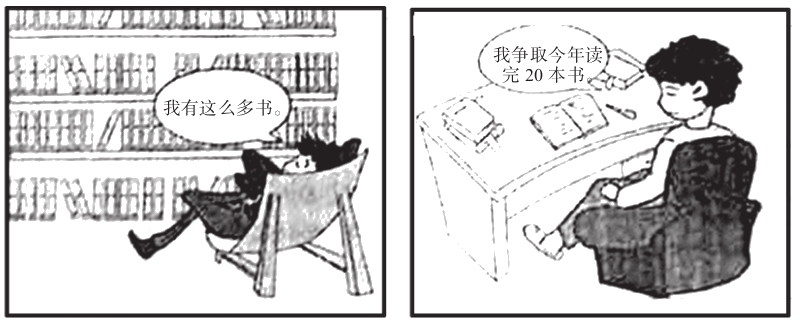
\includegraphics[width=0.87\linewidth]{picture/2017.png}
	\caption*{“有书”与“读书”}
\end{figure}



